\RequirePackage{plautopatch}
\documentclass[uplatex,dvipdfmx,a4paper]{jsarticle}
\usepackage{ics-thesis}

% ===== Other packages =========================================================
\usepackage{otf}
\usepackage[hiresbb]{graphicx}
\usepackage{url}
\usepackage{multirow}
\usepackage{amssymb}
\usepackage{array}
\usepackage{arydshln}
\usepackage{multirow}
\usepackage{listings}
\usepackage[svgnames]{xcolor}
\usepackage{lscape}
\usepackage[caption=false,font=footnotesize]{subfig}
\usepackage{dblfloatfix}
\usepackage{ascmac}
\usepackage{xspace}  % for cite

% ==============================================================================

% ===== Package settings =========================================================
\definecolor{diffstart}{named}{Grey}
\definecolor{diffincl}{named}{Green}
\definecolor{diffrem}{named}{Red}

\lstdefinelanguage{diff}{
  basicstyle=\ttfamily\footnotesize\color{darkgray},
  frame=single,
  linewidth=1.00\textwidth,
  morecomment=[f][\color{diffstart}]{@@},
  morecomment=[f][\color{diffincl}]{+},
  morecomment=[f][\color{diffrem}]{-},
}
\lstset{
  language=diff,
  basicstyle=\ttfamily\footnotesize\color{darkgray},
  frame=single,
  linewidth=1.00\textwidth,
  breaklines=true,
  keywordstyle=\textbf,
  commentstyle=\color{green},
  keywordstyle=\color{blue},
  stringstyle=\color{red},
  tabsize=2,
  lineskip=-0.3zw
}

\hdashlinewidth=0.5pt
\hdashlinegap=1.0pt
% ==============================================================================


% リファレンス参照コマンド
\newcommand{\figref}[1]{図~\ref{#1}}
\newcommand{\tabref}[1]{表~\ref{#1}}
\newcommand{\chapref}[1]{\ref{#1}~章}
\newcommand{\secref}[1]{\ref{#1}~節}
\newcommand{\subsecref}[1]{\ref{#1}~項}

% ハイライトコマンド
\newcommand{\unmodified}[1]{{\textcolor{red}{#1}}}
\newcommand{\modified}[1]{{\textcolor{blue}{#1}}}
\newcommand{\needChange}[1]{{\textcolor{magenta}{#1}}}
\newcommand{\comment}[1]{{\textcolor{darkgray}{#1}}}
\newcommand{\TODO}[1]{{\textcolor{green}{#1}}}
% red,green,blue,cyan,magenta,yellow,black,gray,white,darkgray,lightgray,brown,lime,olive,orange,pink,purple,teal,violet

% footnote用のカウンタ
\newcounter{fcounter}
\setcounter{fcounter}{1}
\newcommand{\fcount}{\the\value{fcounter}\stepcounter{fcounter}}
\newcommand{\fcountin}{\the\value{fcounter}}

\let\oldcite\cite
\renewcommand{\cite}[1]{\xspace\oldcite{#1}}

% ===== Title page configuration ===============================================
\pagestyle{bachelorthesis}
\title{遺伝的アルゴリズムの時間的情報拡張による \\ 時間的効率の調査}
\author{皆森 祐希}
\supervisor{楠本 真二 教授}
\deadline{令和5年2月14日}
% ==============================================================================

\begin{document}

\titlepage

\pagestyle{empty}
\abstract {
  ソフトウェア開発における自動プログラム修正は開発工数の半分を占める作業といわれているデバッグの工数を削減することが期待されており,研究が盛んにおこなわれている.
  自動プログラム修正は,バグを含むプログラムに変更を加えることで用意したテストを通過するプログラムを出力する手法である.
  自動プログラム修正の手法として,遺伝的アルゴリズムに基づいて修正を行うものがある.
  ここで,自動プログラム修正における遺伝的アルゴリズムは,目的のプログラムが得られるまでプログラム文の挿入,削除,置換及び交叉を行う手法である.
  現状の自動プログラム修正における課題の1つとして,1つのプロジェクトに対する実行時間が個体を生成するのにかかった時間を
%Macawは,遺伝的アルゴリズムを採用したAPRツールのひとつであるkGenProgの進化過程をツリー状に可視化するツールであり,遺伝アルゴリズムにおける膨大な変異プログラムの解析を容易にすることが期待される.しかし,kGenProg及びMacawには個体の生成時間を計測および表示する機能が実装されておらず,解となる経路が最適に生成されているかどうかを確かめることが困難である.
  そこで,本研究では遺伝的アルゴリズムを採用したAPRツールのひとつであるkGenProgに各個体の生成にかかった時間を計測する処理を追加し,得られた個体情報をビルドの成否および解であるかどうかに分類し,それらを定量的に調べることで全体の生成時間のうち解となるプログラムの生成経路にかかった時間およびビルドに失敗した個体に費やした時間を計算することで,自動プログラム修正の時間的効率性を調査した.
}

\keyword {
  自動プログラム修正, 時間計測,可視化,  JSON
}

% 目次
\clearpage
\pagestyle{plain}
\pagenumbering{roman}
\tableofcontents

% 図目次
\clearpage
\listoffigures

% 表目次
\clearpage
\listoftables

% 本文
\clearpage
\pagenumbering{arabic}

\newcommand{\kgp}{kGenProg}
\newcommand{\mcw}{Macaw}
%%%%%%%%%%%%%%%%%%%%%%%%%%%%%%%%%%%%%%%%%%%%%%%%%%%%%%%%%%%%%%%%%%%%%%%%%%%%%%%%%%%%%%%%%%%%%%%%%%%
\clearpage
\section{はじめに}\label{sec:intro}
ソフトウェア開発におけるデバッグ作業は費用および時間的な点で多くのコストを必要とする.ある研究によると,ソフトウェア開発にかかるコストのうち,50\%以上をデバッグが占めるという結果が出ている\cite{5386906, Britton_reversibledebugging}.
自動プログラム修正(APR)は,人の手を介さずにソースコード中に含まれるバグを全自動で取り除く技術であり,盛んに研究が進められている\cite{gazzola2018automatic, goues2019automated}.
%APRは大きく探索ベースの手法と意味論ベースの2つの手法に分類することができるが,本研究では,探索ベース
APRの実用化に向けて,ここ10年で数多くの研究がなされており,時間的なコストを削減する取り組みが数多く行われている\cite{id692}.\TODO{TODO : 時間的コスト削減についての追加の論文調査}しかし,先行研究においては個体の生成時間に関する研究は多くない.そこで,本稿では,既存のAPRツールを拡張して個体の生成時間を計測し,独自の指標を実際のバグに対して計算することで時間的コストを調査する.\\
以降,\ref{sec:prep}章ではAPRの課題本研究を行う契機となった研究の説明および研究のための予備知識について説明する.\\
\ref{sec:prop}章では今回提案した評価指標とその具体例について論述する.\\
\ref{sec:exp}章では実験の概要と結果を提示する.\\
\ref{sec:cons}章では実験から得られた結果による考察について述べる.\\
\ref{sec:threat}章では本研究の妥当性への脅威について論じる.\\
\ref{sec:ftrclg}章では今後の課題について説明し,\\
最後に\ref{sec:concl}章で総括を述べる.
%%%%%%%%%%%%%%%%%%%%%%%%%%%%%%%%%%%%%%%%%%%%%%%%%%%%%%%%%%%%%%%%%%%%%%%%%%%%%%%%%%%%%%%%%%%%%%%%%%%

\clearpage
\section{準備}\label{sec:prep}
本章では,遺伝的アルゴリズム(GA)に基づく自動プログラム修正(APR) の生成過程について述べる.
\subsection{自動プログラム修正(APR)}\label{sec:apr}
APRは,テストケースと空プログラムを入力として,計算機が自動的にプログラムのバグを修正する技術である.APRは大きく探索ベース\footnote{Heuristics-based}と意味論ベース\footnote{Semantics-based}の2つの手法に分類することができるが,本研究では,探索ベースAPR分野のブレイクスルーとなったGenProg\cite{le2011genprog}の採用する生成と検証\cite{martinez2019astor}に基づく手法に重点を置く.\\
この手法では,図\ref{fig:apr}\TODO{TODO : 図を用いて詳述する}のように,対象となるプログラムにおけるバグの位置を特定する欠陥限局を行い,限局した箇所に変更を加えた後ビルドとテストを実行することで修正できたかどうかの評価を行う.
\subsection{遺伝的アルゴリズム}\label{sec:ga}
遺伝的アルゴリズム(GA)は各世代で個体を選択し,それらに変異,交叉などの操作を加えることでより強い個体を生成する生物の進化に基づくアルゴリズムである.
\\\TODO{TODO : 図を用いて詳述する}
具体的に説明すると,ある世代において,図\ref{fig:ga}のような個体があったとする.これらの個体から以下の遺伝子操作を行う.
\begin{description}
\item{選択} …個体のうちから何らかの関数による適応度(APRではテストスイートの通過率)に応じて選択
\item{変異} …個体の遺伝子を変異させる(APRではコードの一部を変更)
\item{交叉} …複数の遺伝子の一部分を交配させて新しい遺伝子を生成
\end{description}
APRでは,変異において以下の操作を行う.
\begin{description}
\item{挿入} …選択したコードの近辺に別のコードを追加する
\item{置換} …選択したコードを別のコードに書き換える
\item{交叉} …選択したコードを削除する
\end{description}
\subsection{既存のAPRツールの課題} \label{sec:prev_challenge}
既存のAPRツールは多くの課題が解決されておらず\cite{le2013current},まだまだ実用には程遠い段階である.具体的には,修正後のプログラムの可読性が低い\cite{smith2015cure},\\
その中で今回主に取り上げる課題として,1回の修正実行にビルドやテスト実行といった多くの時間的コストがかかる点\cite{chen2017contract}があげられる.
また,先行研究においては,ビルドとテストにかかる時間を削減する研究が行われているものの\cite{id692}
%テストの実行時間を計測する機能は実装されているものの
,個体の生成そのものにかかった時間を計測する機能に関する研究はまだ発展途上である.
\subsection{時間的コスト調査の先行研究}
Ghanbari\cite{ghanbari2019practical}らはソースコードレベルのAPRに加えて,さらにバイトコードにAPRを施すPraPRを提案し,既存のAPRの性能を飛躍的に向上させた.この研究において,提案したPraPRをDefects4JのChartおよびClosureバグに対して時間的コストを計算した.結果として,Closureバグでは有効なパッチの数がChartバグに比べて10倍生成されたものの,時間的コストは20倍かかった.
また,古藤\cite{id692}らは欠陥限局を用いて変更コード片を動的に切り替える手法を提案しビルドに費やす時間を従来手法に比べて89\%から46\%に削減することができ,結果としてAPR全体の修正時間の削減につながった.
これらの研究をきっかけとして,自動プログラム修正の時間的コストについてより詳らかに調べてみようと思い,本研究をするに至った.

%%%%%%%%%%%%%%%%%%%%%%%%%%%%%%%%%%%%%%%%%%%%%%%%%%%%%%%%%%%%%%%%%%%%%%%%%%%%%%%%%%%%%%%%%%%%%%%%%%%
\clearpage
\section{評価指標とその実装} \label{sec:prop}
\subsection{評価指標}\label{sec:index}
\subsubsection{STR}\label{sec:STR}
APRを実行するにあたり,修正に成功したプロジェクトに対して,その解となる個体に関係する経路の全体の生成時間に占める割合を求める指標として,{\bf STR}(Solution Time Ratio, 解時間比率)を式\label{eq:STR}で定義する.
\begin{equation}
\label{eq:STR} {\rm STR} =  \frac{解となる個体の経路の総生成時間}{すべての個体の総生成時間}
\end{equation}
ここで,解となる個体の経路の集合は
\begin{enumerate}
\item まず解である個体を選択し,集合に入れる \label{sol:step1}
\item 集合内の全個体に対してその親を求め,それらを集合に入れる \label{sol:step2}
\item 集合に変化がなくなるまで\ref{sol:step2}を繰り返す \label{sol:step3}
\end{enumerate}
のように求められる.STRを計算する目的として,プログラム修正において成功に必要な個体の生成が時間的にどの程度の割合を占めているのかを定量的に求めることがあげられる.そのため,STRの値は大きい方が好ましい.
\subsubsection{FTR}\label{sec:FTR}
一方で,すべてのプロジェクトに対してビルドに失敗する個体がすべての個体の生成時間に占める割合を求める指標として,{\bf FTR}(Failure Time Ratio, 失敗時間比率)を式\label{eq:FTR}で定義する.
\begin{equation}
\label{eq:FTR} {\rm FTR} =  \frac{ビルドに失敗した個体にかかった総生成時間}{すべての個体の総生成時間}
\end{equation}
FTRを計算する目的として,プロジェクト内のプログラムの修正にかかる時間のうちがどの程度の割合を占めるかを定量的に測定し,その傾向を知ることがあげられる.そのため,一般的にFTRの値は小さい方が望ましいとされる.
\subsection{STR・FTRの具体的な計算例}
先ほど定義した値を求めるための具体的な例として,図\ref{fig:example}の生成木をもつ修正結果について考える.この生成木は,kGenProgの実行結果を記したJSONファイルをツリー状に表示する\mcw \cite{tomida2019visualizing}を参考に描画した\footnote{X印における数字の意味合いが違うなど細かい違いがある点に注意}.
\begin{figure}[t]
  \centering
  \includegraphics[width=\linewidth]{fig/astSample.pdf}
  \caption{生成結果の例}
  \label{fig:example}
\end{figure}
ここで,縦方向は世代を表しており,下に進むにつれてより新しい世代を表す.また,横の列は一つの世代におけるすべての個体を表す.円及びX印はそれぞれビルドに成功した1つの個体,その世代でビルドに失敗したすべての個体を表す.円の色は個体のFitness(全体のテストケースに占める期待通りのテスト結果が得られた割合)を表し,緑に近いほど高いFitnessを右下の数字はその個体あるいは個体の集合の生成時間を表す.なおこの例におけるプログラムの総生成時間は800である.
この時,STRは図\ref{fig:example_STR}で表される部分の時間$(10 + 15 + 5 + 100 + 200) \div 800 = 0.4125$となり,FTRはX印で示されたすべての時間を足した値を総生成時間で割ったもの,すなわち$(150 + 250) \div 800 = 0.5$と求められる.
\begin{figure}[t]
  \centering
  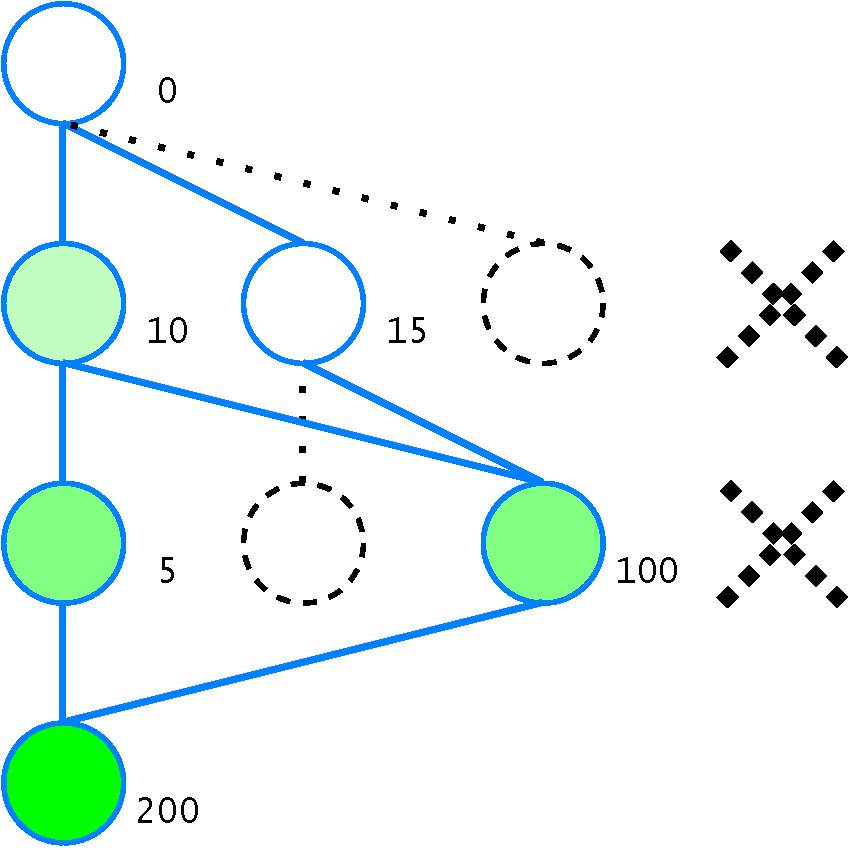
\includegraphics[width=\linewidth]{fig/astSample_STR.pdf}
  \caption{生成結果の例}
  \label{fig:example_STR}
\end{figure}
\subsection{APRツールへの時間計測機能実装} \label{sec:impl}
提案手法では,既存のAPRツールであるkGenProg\cite{higo2018kgenprog}を拡張して実装する.
ソースコード内部のふるまいは変えずに,\texttt{Mutation}クラスと\texttt{RandomCrossover}クラスに時間計測を行うコードを挿入した.具体的には,\texttt{org.apache.commons.lang3.time.StopWatch}クラスをインポートし,各個体を生成するループの最初に\texttt{StopWatch.createStarted()}メソッドを呼び出すことによって時間計測を開始,処理を終えた後に\texttt{getTime()}メソッドを呼び出すことで生成時間を取得し,それを個体情報に格納する.この際,kGenProgに付属しているJSONファイルの出力オプションをオンにすることで,プロジェクトにおける個体の解析を可能にする.\\
次に,JSONファイルをPythonで記述したプログラムを用いて処理し,各個体のID(通し番号)・生成時間・Fitness(ただしここではIDに対応する個体がビルドに失敗した場合-1を格納する)の情報を取得した後,その情報をもとにSTRとFTRを計算する.\\
具体的には,出力となるJSONファイルを読み込み,そのプロジェクトで生成された個体の時間を1つずつ取得する.この時,Fitnessの値で追加の処理を行う.例えばFitnessが-1であればビルドに失敗した個体であるので失敗時間(FTRを計算する際の分子)に加算する.また,Fitnessが1であれば,テストケースを満たす解となる個体であるので\ref{sec:STR}で挙げた手順で解となる個体の親を求める.プログラム中では再帰的なアルゴリズムを用いている.\\
%%%%%%%%%%%%%%%%%%%%%%%%%%%%%%%%%%%%%%%%%%%%%%%%%%%%%%%%%%%%%%%%%%%%%%%%%%%%%%%%%%%%%%%%%%%%%%%%%%%
\clearpage
\section{実験} \label{sec:exp}
\subsection{概要}
本章では,GAを採用したAPRツールであるkGenProg\cite{higo2018kgenprog}を用いて,Defects4J\cite{just2014defects4j}のLangプロジェクトのLang1~Lang44を対象に自動プログラム修正を行った.そのうち,ビルドに成功し,かつ解を得ることができたLang6, 
%Lang10,
 Lang22, Lang25およびLang39の
%5
4つのプロジェクトを対象として先ほど定義したSTRとFTRを計算し,その値を確認する.なお,生成時間には不確定性があるため各プロジェクトごとにAPRを複数回実行している.
表\ref{tab:apr_setting}にAPRツール実行時の設定を,表\ref{tab:project_setting}に実行回数や解に至るまでの総個体数など,各プロジェクトに対する実験の条件を示す.
\begin{table}[b]
  \centering
  \caption{APRツールの設定}
  \label{tab:apr_setting}
  \begin{tabular}{ll} \hline\hline
    項目         & 値                           \\\hline
    実験題材     & Defects4J Lang6, Lang22, Lang25, Lang39 \\
    題材数       & 4                           \\
    乱数シード   & 2       \\\\
    実験環境     & Corei5-1240P 16GB mem  \\\hline\hline
  \end{tabular}
\end{table}
\begin{table}[b]
  \centering
  \caption{各プロジェクトの詳細}
  \label{tab:project_setting}
  \begin{tabular}{lllll} \hline\hline
    プロジェクト名 & Lang6 & Lang22 & Lang25 & Lang39  \\\hline
    到達世代数 & 1 & 7 & 1 & 4 \\
    個体数 & 8 & 624 & 38 & 300 \\
    ビルド失敗個体数 & 7 & 511 & 36 & 274 \\
    サンプル数 & 100 & 15 & 70 & 40 \\\hline\hline
  \end{tabular}
\end{table}
ここで,サンプル数がプロジェクトによって異なるのは,1回のプログラム修正にかかる総時間が異なるためである.
\subsection{実験結果}
\TODO{ここもう少し詳細に書く¥}
\subsubsection{Lang6}
図\ref{fig:Lang6_boxplot}にLang6におけるSTRとFTRの箱ひげ図を,表\ref{tab:Lang6}にSTRとFTRの平均(以降AVG),最小値(以降MIN),第1四分位数(以降1Q),中央値(以降MED),第3四分位数(以降3Q),最大値(以降MAX)の各データを示す.
\begin{figure}[t]
  \centering
  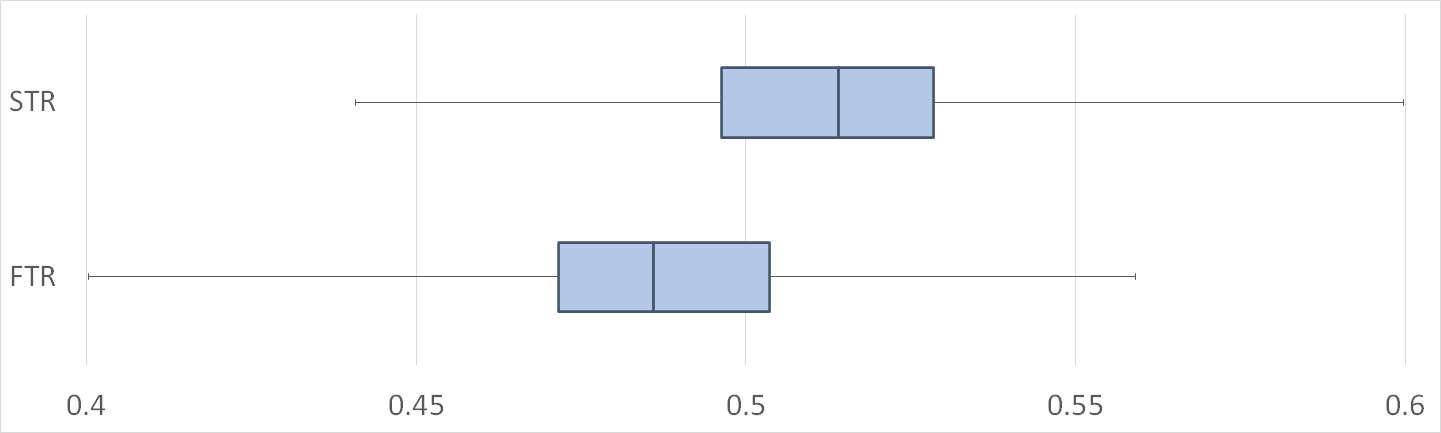
\includegraphics[width=\linewidth]{fig/Lang6_boxplot.png}
  \caption{箱ひげ図 : Lang6}
  \label{fig:Lang6_boxplot}
\end{figure}
\begin{table}[b]
  \centering
  \caption{Lang6プロジェクトのSTR, FTR}
  \label{tab:Lang6}
  \begin{tabular}{l|llllll} \hline\hline
    評価指標 & AVG         & MIN & 1Q & MED & 3Q & MAX   \\\hline
    STR & 0.5117 & 0.4409 & 0.4964 & 0.5140 & 0.5284 & 0.5997  \\
    FTR & 0.4883 & 0.4003 & 0.4716 & 0.4860 & 0.5036 & 0.5591 \\\hline\hline
  \end{tabular}
\end{table}
\begin{figure}[t]
  \centering
  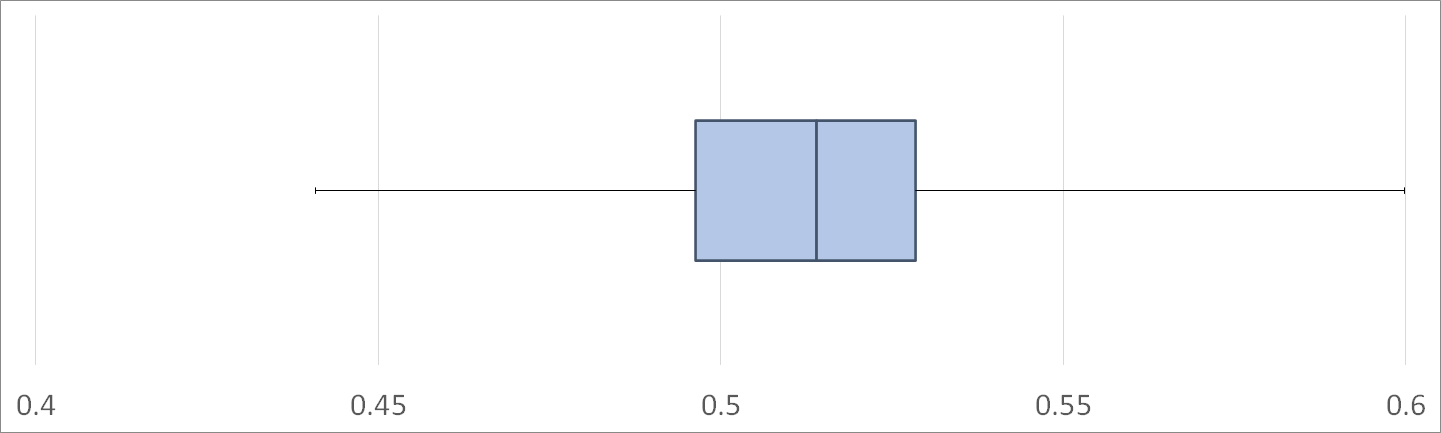
\includegraphics[width=\linewidth]{fig/Lang6_boxplot_STR.png}
  \caption{STRの箱ひげ図 : Lang6}
  \label{fig:Lang6_boxplot_STR}
\end{figure}
\begin{figure}[t]
  \centering
  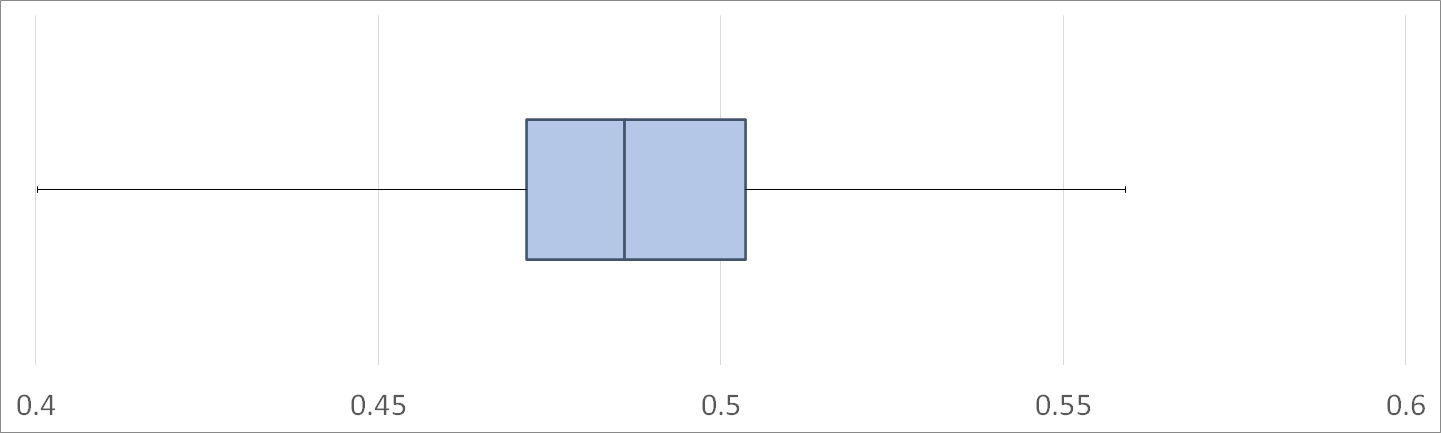
\includegraphics[width=\linewidth]{fig/Lang6_boxplot_FTR.png}
  \caption{FTRの箱ひげ図 : Lang6}
  \label{fig:Lang6_boxplot_FTR}
\end{figure}
\subsubsection{Lang22}
図\ref{fig:Lang22_boxplot}にLang22におけるSTRとFTRの箱ひげ図を示す.
\begin{figure}[t]
  \centering
  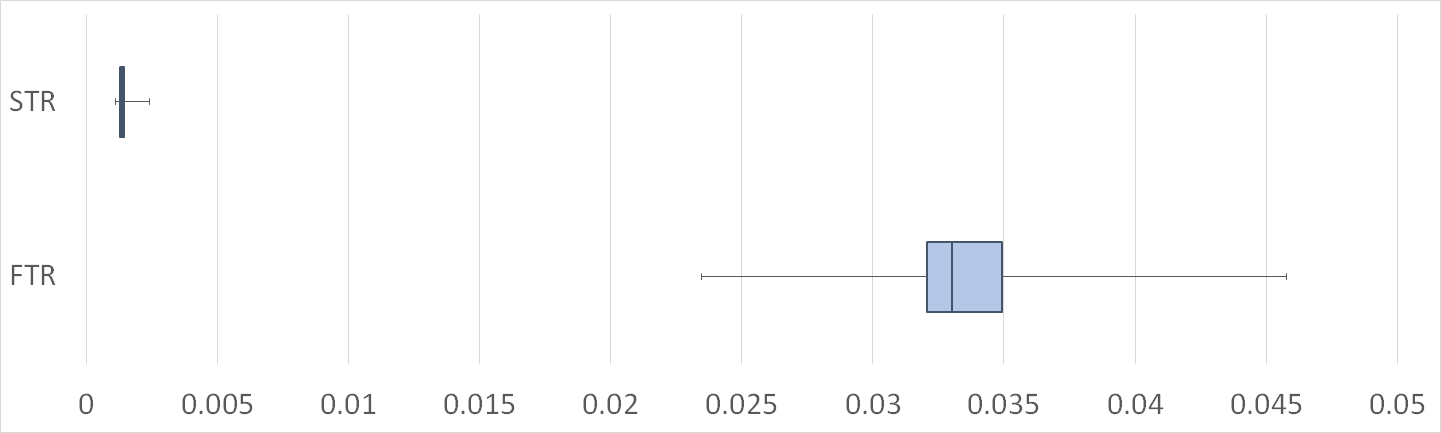
\includegraphics[width=\linewidth]{fig/Lang22_boxplot.png}
  \caption{箱ひげ図 : Lang22}
  \label{fig:Lang22_boxplot}
\end{figure}
\begin{table}[b]
  \centering
  \caption{Lang22プロジェクトのSTR, FTR}
  \label{tab:Lang22}
  \begin{tabular}{l|llllll} \hline\hline
    評価指標 & AVG         & MIN & 1Q & MED & 3Q & MAX   \\\hline
    STR & 0.001476 & 0.001096 & 0.001291 & 0.001354 & 0.001458 & 0.002418  \\
    FTR & 0.03432 & 0.02346 & 0.03208 & 0.03304 & 0.03492 & 0.04578 \\\hline\hline
  \end{tabular}
\end{table}
\begin{figure}[t]
  \centering
  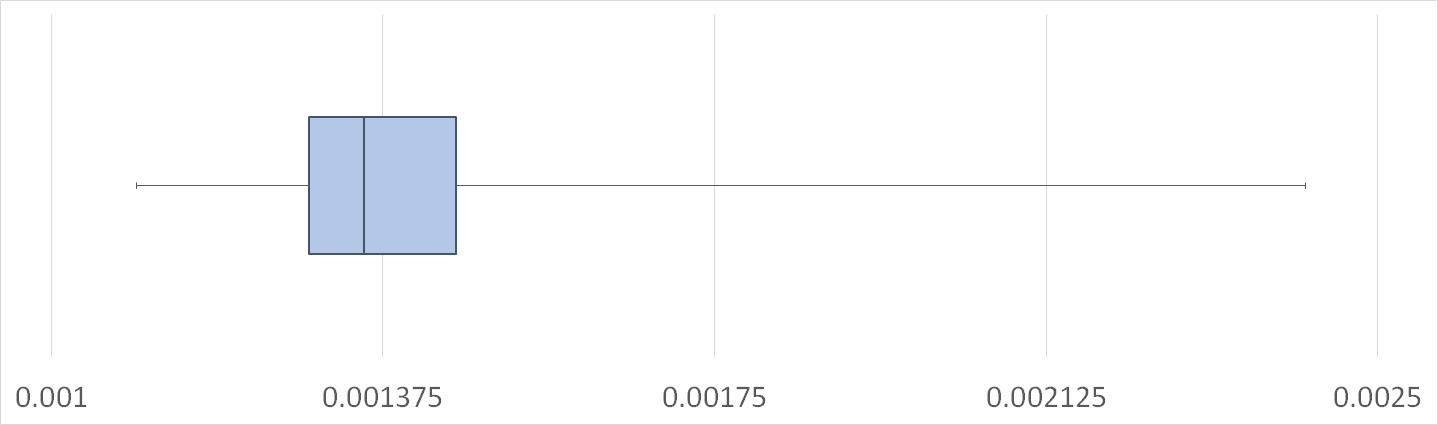
\includegraphics[width=\linewidth]{fig/Lang22_boxplot_STR.png}
  \caption{STRの箱ひげ図 : Lang22}
  \label{fig:Lang22_boxplot_STR}
\end{figure}
\begin{figure}[t]
  \centering
  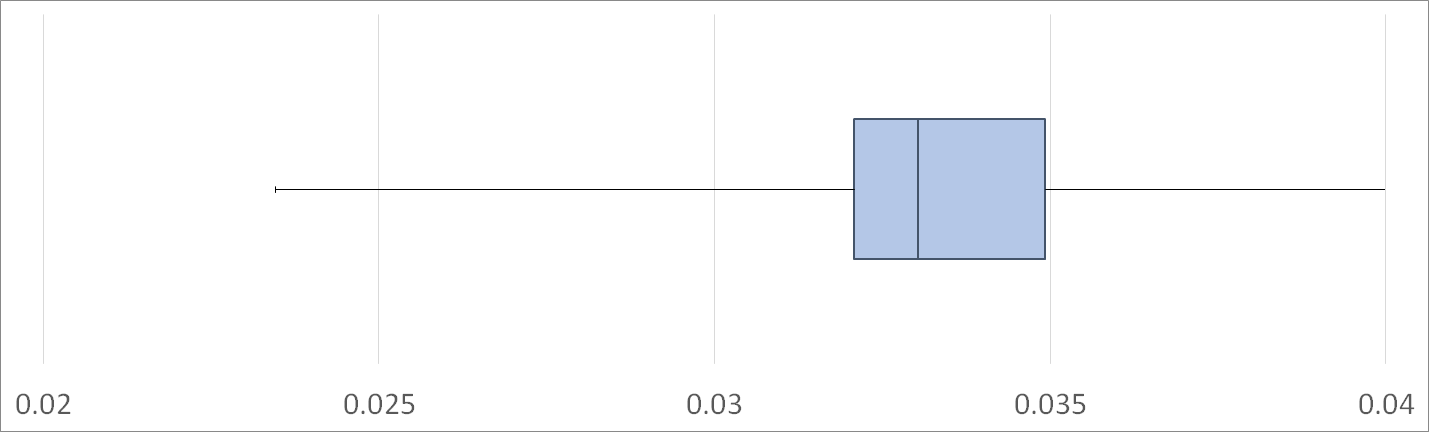
\includegraphics[width=\linewidth]{fig/Lang22_boxplot_FTR.png}
  \caption{FTRの箱ひげ図 : Lang22}
  \label{fig:Lang22_boxplot_FTR}
\end{figure}
\subsubsection{Lang25}
図\ref{fig:Lang25_boxplot}にLang25におけるSTRとFTRの箱ひげ図を示す.
\begin{figure}[t]
  \centering
  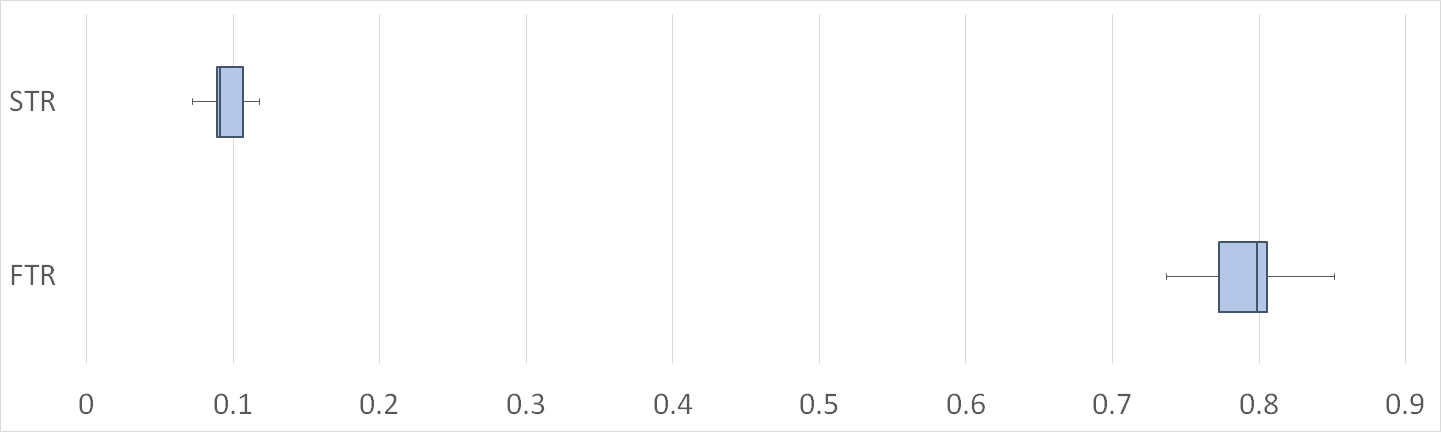
\includegraphics[width=\linewidth]{fig/Lang25_boxplot.png}
  \caption{箱ひげ図 : Lang25}
  \label{fig:Lang25_boxplot}
\end{figure}
\begin{table}[b]
  \centering
  \caption{Lang25プロジェクトのSTR, FTR}
  \label{tab:Lang25}
  \begin{tabular}{l|llllll} \hline\hline
    評価指標 & AVG         & MIN & 1Q & MED & 3Q & MAX   \\\hline
    STR & 0.09386 & 0.07261 & 0.08936 & 0.09106 & 0.1070 & 0.1177  \\
    FTR & 0.7986 & 0.7371 & 0.7725 & 0.7989 & 0.8053 & 0.8512 \\\hline\hline
  \end{tabular}
\end{table}
\begin{figure}[t]
  \centering
  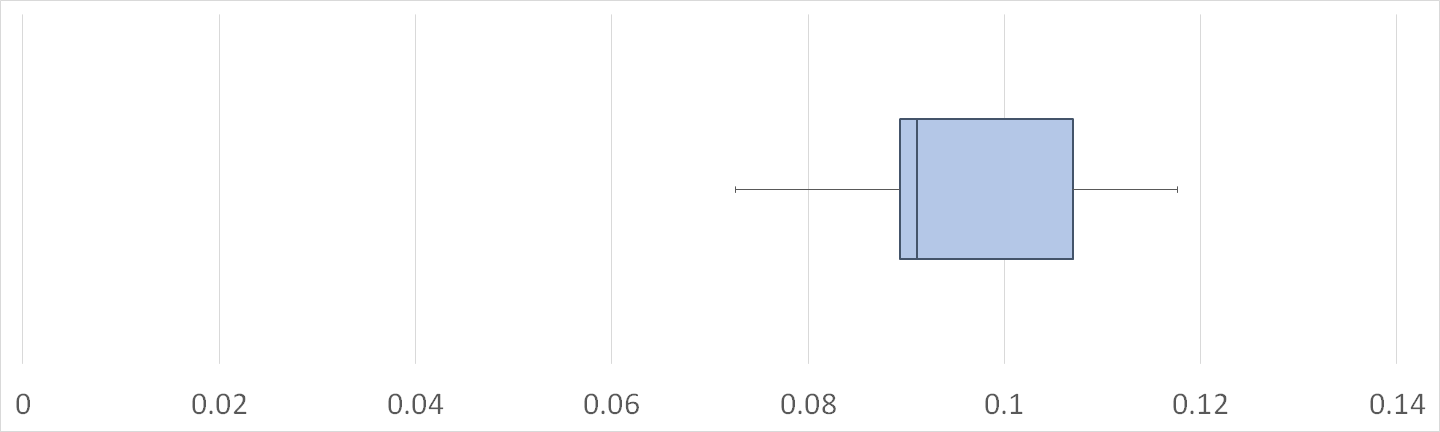
\includegraphics[width=\linewidth]{fig/Lang25_boxplot_STR.png}
  \caption{STRの箱ひげ図 : Lang25}
  \label{fig:Lang25_boxplot_STR}
\end{figure}
\begin{figure}[t]
  \centering
  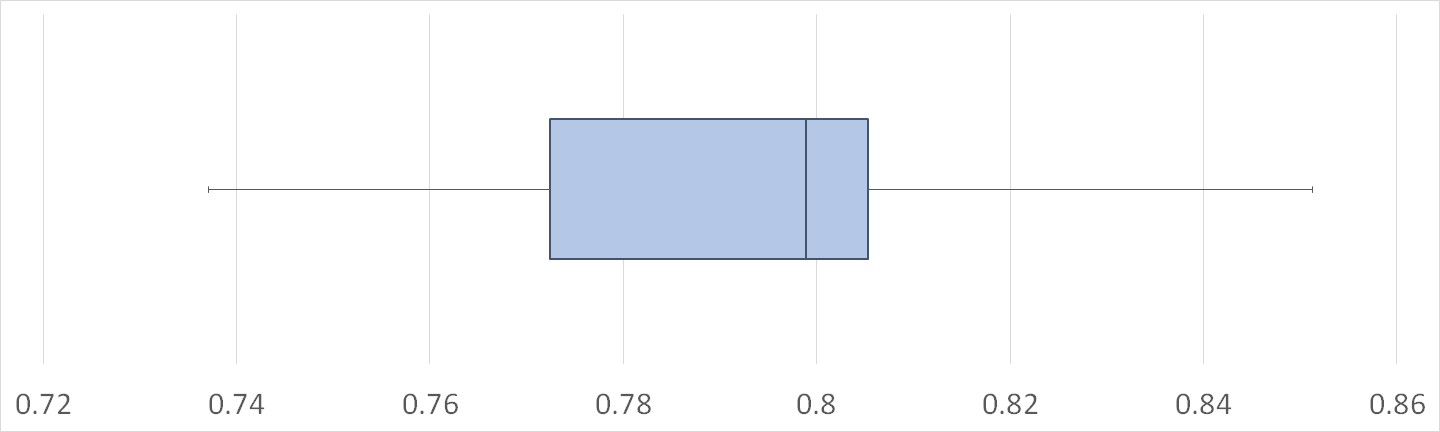
\includegraphics[width=\linewidth]{fig/Lang25_boxplot_FTR.png}
  \caption{FTRの箱ひげ図 : Lang25}
  \label{fig:Lang25_boxplot_FTR}
\end{figure}
\subsubsection{Lang39}
図\ref{fig:Lang39_boxplot}にLang39におけるSTRとFTRの箱ひげ図を示す.
\begin{figure}[t]
  \centering
  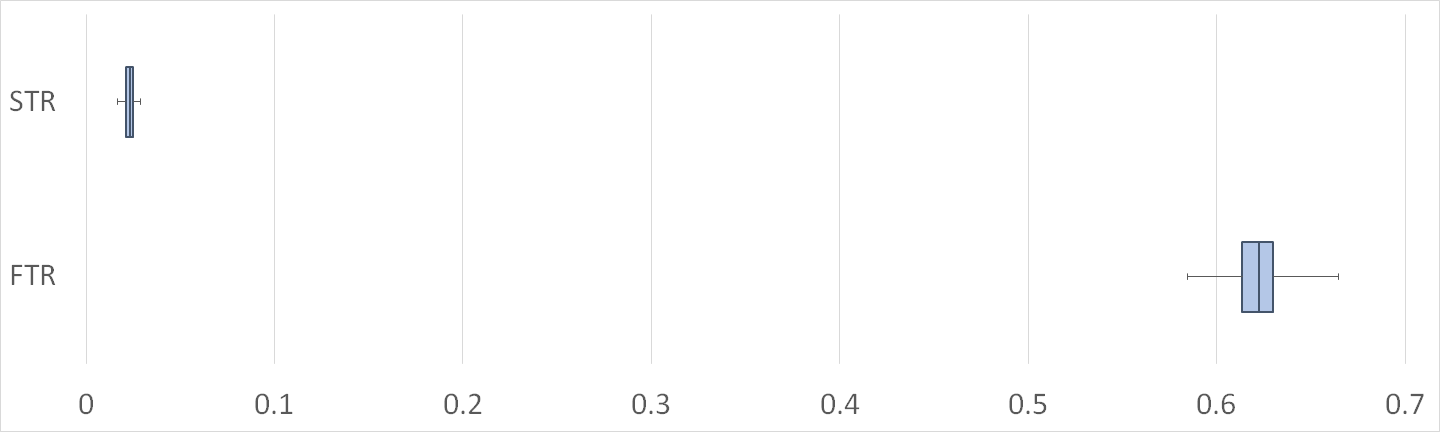
\includegraphics[width=\linewidth]{fig/Lang39_boxplot.png}
  \caption{箱ひげ図 : Lang39}
  \label{fig:Lang39_boxplot}
\end{figure}
\begin{table}[b]
  \centering
  \caption{Lang39プロジェクトのSTR, FTR}
  \label{tab:Lang39}
  \begin{tabular}{l|llllll} \hline\hline
    評価指標 & AVG         & MIN & 1Q & MED & 3Q & MAX   \\\hline
    STR & 0.02406 & 0.01645 & 0.02105 & 0.02326 & 0.02510 & 0.02873  \\
    FTR & 0.6218 & 0.5847 & 0.6137 & 0.6224 & 0.6299 & 0.6644 \\\hline\hline
  \end{tabular}
\end{table}
\begin{figure}[t]
  \centering
  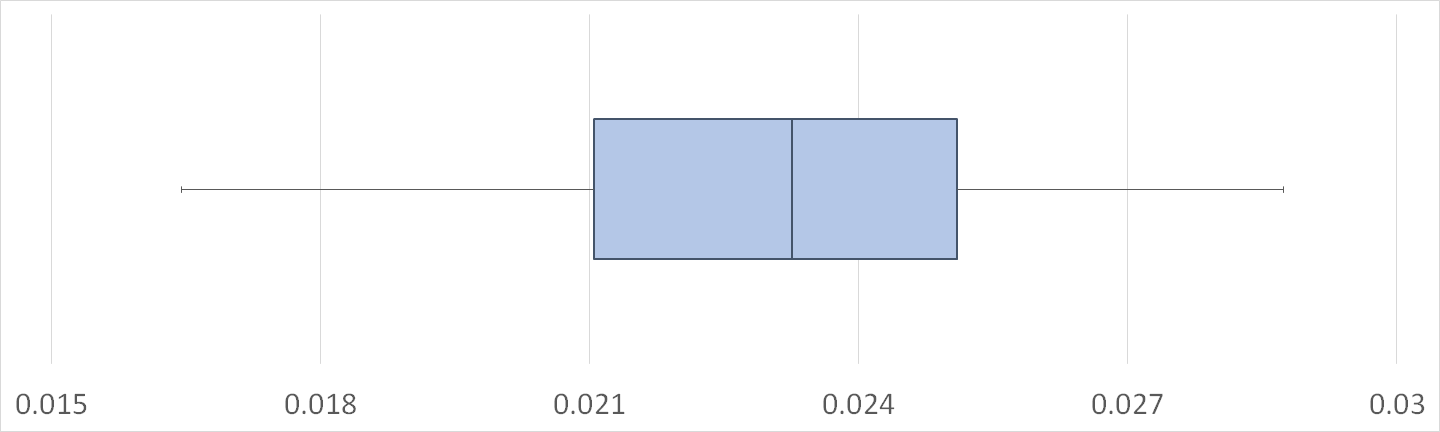
\includegraphics[width=\linewidth]{fig/Lang39_boxplot_STR.png}
  \caption{STRの箱ひげ図 : Lang39}
  \label{fig:Lang39_boxplot_STR}
\end{figure}
\begin{figure}[t]
  \centering
  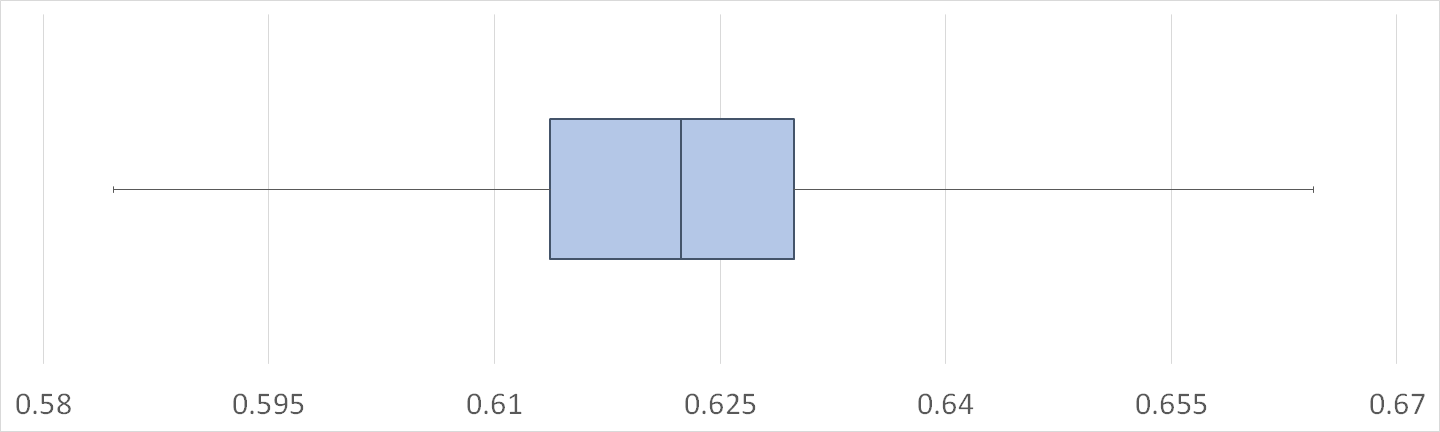
\includegraphics[width=\linewidth]{fig/Lang39_boxplot_FTR.png}
  \caption{FTRの箱ひげ図 : Lang39}
  \label{fig:Lang39_boxplot_FTR}
\end{figure}
%%%%%%%%%%%%%%%%%%%%%%%%%%%%%%%%%%%%%%%%%%%%%%%%%%%%%%%%%%%%%%%%%%%%%%%%%%%%%%%%%%%%%%%%%%%%%%%%%%%
\clearpage
\section{考察}\label{cons}
次に,\ref{sec:exp}章で行った実験の結果から,各プロジェクトおよび全体的なSTRとFTRの傾向について考察する.
まず,Lang6プロジェクトについて述べる.修正を完了するまでに生成した個体の数が8つと比較的少ないこともあってか,
次に,Lang22プロジェクトの修正においては,他のプロジェクトの修正により多くの時間および操作を要した.そのため,他のプロジェクトに比べるとSTR,FTRのいずれの値も小さくなっている.ついで,Lang25プロジェクトの特徴として,


%%%%%%%%%%%%%%%%%%%%%%%%%%%%%%%%%%%%%%%%%%%%%%%%%%%%%%%%%%%%%%%%%%%%%%%%%%%%%%%%%%%%%%%%%%%%%%%%%%%
\clearpage
\section{妥当性の脅威}\label{threat}
\ref{sec:exp}章における実験において考えうる妥当性の脅威について論ずる.この実験では内的要因と外的要因に大別される.
まず内的要因として,今回実行した環境とは異なる環境において実行した際に算出されるSTRとFTRの値が異なる可能性がある点があげられる.また,実行時に他のタスクによりメモリが占領されている場合,普段と異なる値が算出されうる点があげられる.\\
次に外的要因として,大規模なプロジェクトにおいて何万といった個体が生成されたときにSTRとFTRの値が大きく異なる今回対象としたプロジェクトは個体数が多いもので600程度と比較的少なかった.
% また,kGenProg以外のツールを用いて実験を行った場合,
%%%%%%%%%%%%%%%%%%%%%%%%%%%%%%%%%%%%%%%%%%%%%%%%%%%%%%%%%%%%%%%%%%%%%%%%%%%%%%%%%%%%%%%%%%%%%%%%%%%
\clearpage
\section{今後の課題}\label{sec:ftrclg}
\subsection{APRツールによる生成時間の違いの検証}
本研究においては,APRツールとして探索ベースであり,かつ遺伝的アルゴリズムを採用した\kgp を対象に個体の生成時間計測を行ったが,遺伝的アルゴリズムでないほかの探索ベースのAPRツールや意味論ベースのAPRツールにおいて時間計測を行う.
\subsection{時間計測を行う対象プロジェクトの拡張}
本研究では,Defects4JのLangバグのうち,4つのプロジェクトを対象としてSTRとFTRの計算を行った.今後は,Defects4Jのほかのバグやその他の対象について時間研究を行う.
%%%%%%%%%%%%%%%%%%%%%%%%%%%%%%%%%%%%%%%%%%%%%%%%%%%%%%%%%%%%%%%%%%%%%%%%%%%%%%%%%%%%%%%%%%%%%%%%%%%
\clearpage
\section{おわりに}
本稿において,APRツールに個体の生成にかかった時間を計測する

% =================================================================================================
% 謝辞
\clearpage
\acknowledgement

本研究を進めるにあたり,多くの方々からご支援およびご助言を賜りました.

楠本 真二 教授には,本研究を快く快諾し,暖かく見守ってくださりました.
心より感謝申し上げます.

肥後 芳樹 准教授には,議論を重ねに重ね,本研究の完成のご支援及び的確なご助言を賜りました.
心より感謝申し上げます.

柗本 真佑 助教には,テーマが決まらず途方に暮れていた際,鋭くも的確なご助言を賜りました.
深く感謝いたします.

古藤 寛大先輩には,困難に直面した際いつも迅速にご助言を賜り感謝してもしきれません.

本研究に至るまでに,講義,演習等でお世話になりました大阪大学基礎工学部情報科学科の諸先生方に,御礼申し上げます.

最後に,これまでお世話になりました家族,小中高校の教員方,その他すべての方に感謝申し上げます.
% =================================================================================================
% 参考文献
\clearpage
\bibliographystyle{junsrt}
\bibliography{references.bib}

\end{document}
